\section{Numerical equilibrium paths}

\subsection{Benchmark and method}

The numerical experiments are not a calibration exercise. Parameters with
standard macroeconomic counterparts are held fixed, while the two substitution
elasticities define the cases of interest. Table \ref{tab:axm-parameters} reports
the benchmark.

As in the model, raw compute is measured in resource-expenditure units, so its
common unit cost is one and is not a free parameter.

\begin{table}[H]
\centering
\caption{Benchmark parameters}
\label{tab:axm-parameters}
\begin{tabular}{lcl}
\toprule
Parameter & Value & Interpretation\\
\midrule
\(\alpha\) & 0.33 & Capital elasticity in final output\\
\(n\) & 0.012 & Annual population growth\\
\(\delta\) & 0.05 & Annual depreciation\\
\(\rho\) & 0.04 & Household discount rate\\
\(\omega_X\) & 0.20 & AI weight in the final CES\\
\(\omega_M\) & 0.35 & Automated-service weight in research\\
\(\eta\) & 0.45 & Returns to effective research\\
\(\chi\) & 0.01 & Research-productivity normalization\\
\bottomrule
\end{tabular}
\end{table}

Initial \(A\) and \(N\) are normalized to one. Initial capital is chosen near the
limiting capital-output ratio of the unit-elasticity benchmark. The level of
\(\chi\) and the normalizations affect calendar timing, so the very long horizontal
axis should not be read as a forecast. The economically meaningful objects are
the direction of the transition, the limiting rates and shares, and the
comparison across research technologies.

The solver treats \(K\) and \(A\) as predetermined and chooses initial \(C\) and
\(q\) so that the path approaches the relevant terminal equilibrium. At every
collocation node it solves the monopoly supply condition, labor-market clearing,
the dual research problem, both research first-order conditions, and the four
equations in \eqref{eq:axm-canonical-system}.

\subsection{Unit elasticity in final production}

Figure \ref{fig:axm-research-comparison} compares Cobb--Douglas research
\((\sigma_{HM}=1)\) with gross substitution in research
\((\sigma_{HM}=2)\), holding \(\sigma_{XL}=1\). The analytical limits from
Proposition \ref{prop:axm-cd-bgp} are visible. Under Cobb--Douglas research, the
automated contribution is fixed at \(\omega_M=0.35\), capability growth converges
to 0.67 percent, and output-per-capita growth converges to 0.17 percent. With
gross substitution, the automated contribution approaches one, capability growth
converges to 1.23 percent, and output-per-capita growth approaches 0.31 percent.

\begin{figure}[H]
\centering
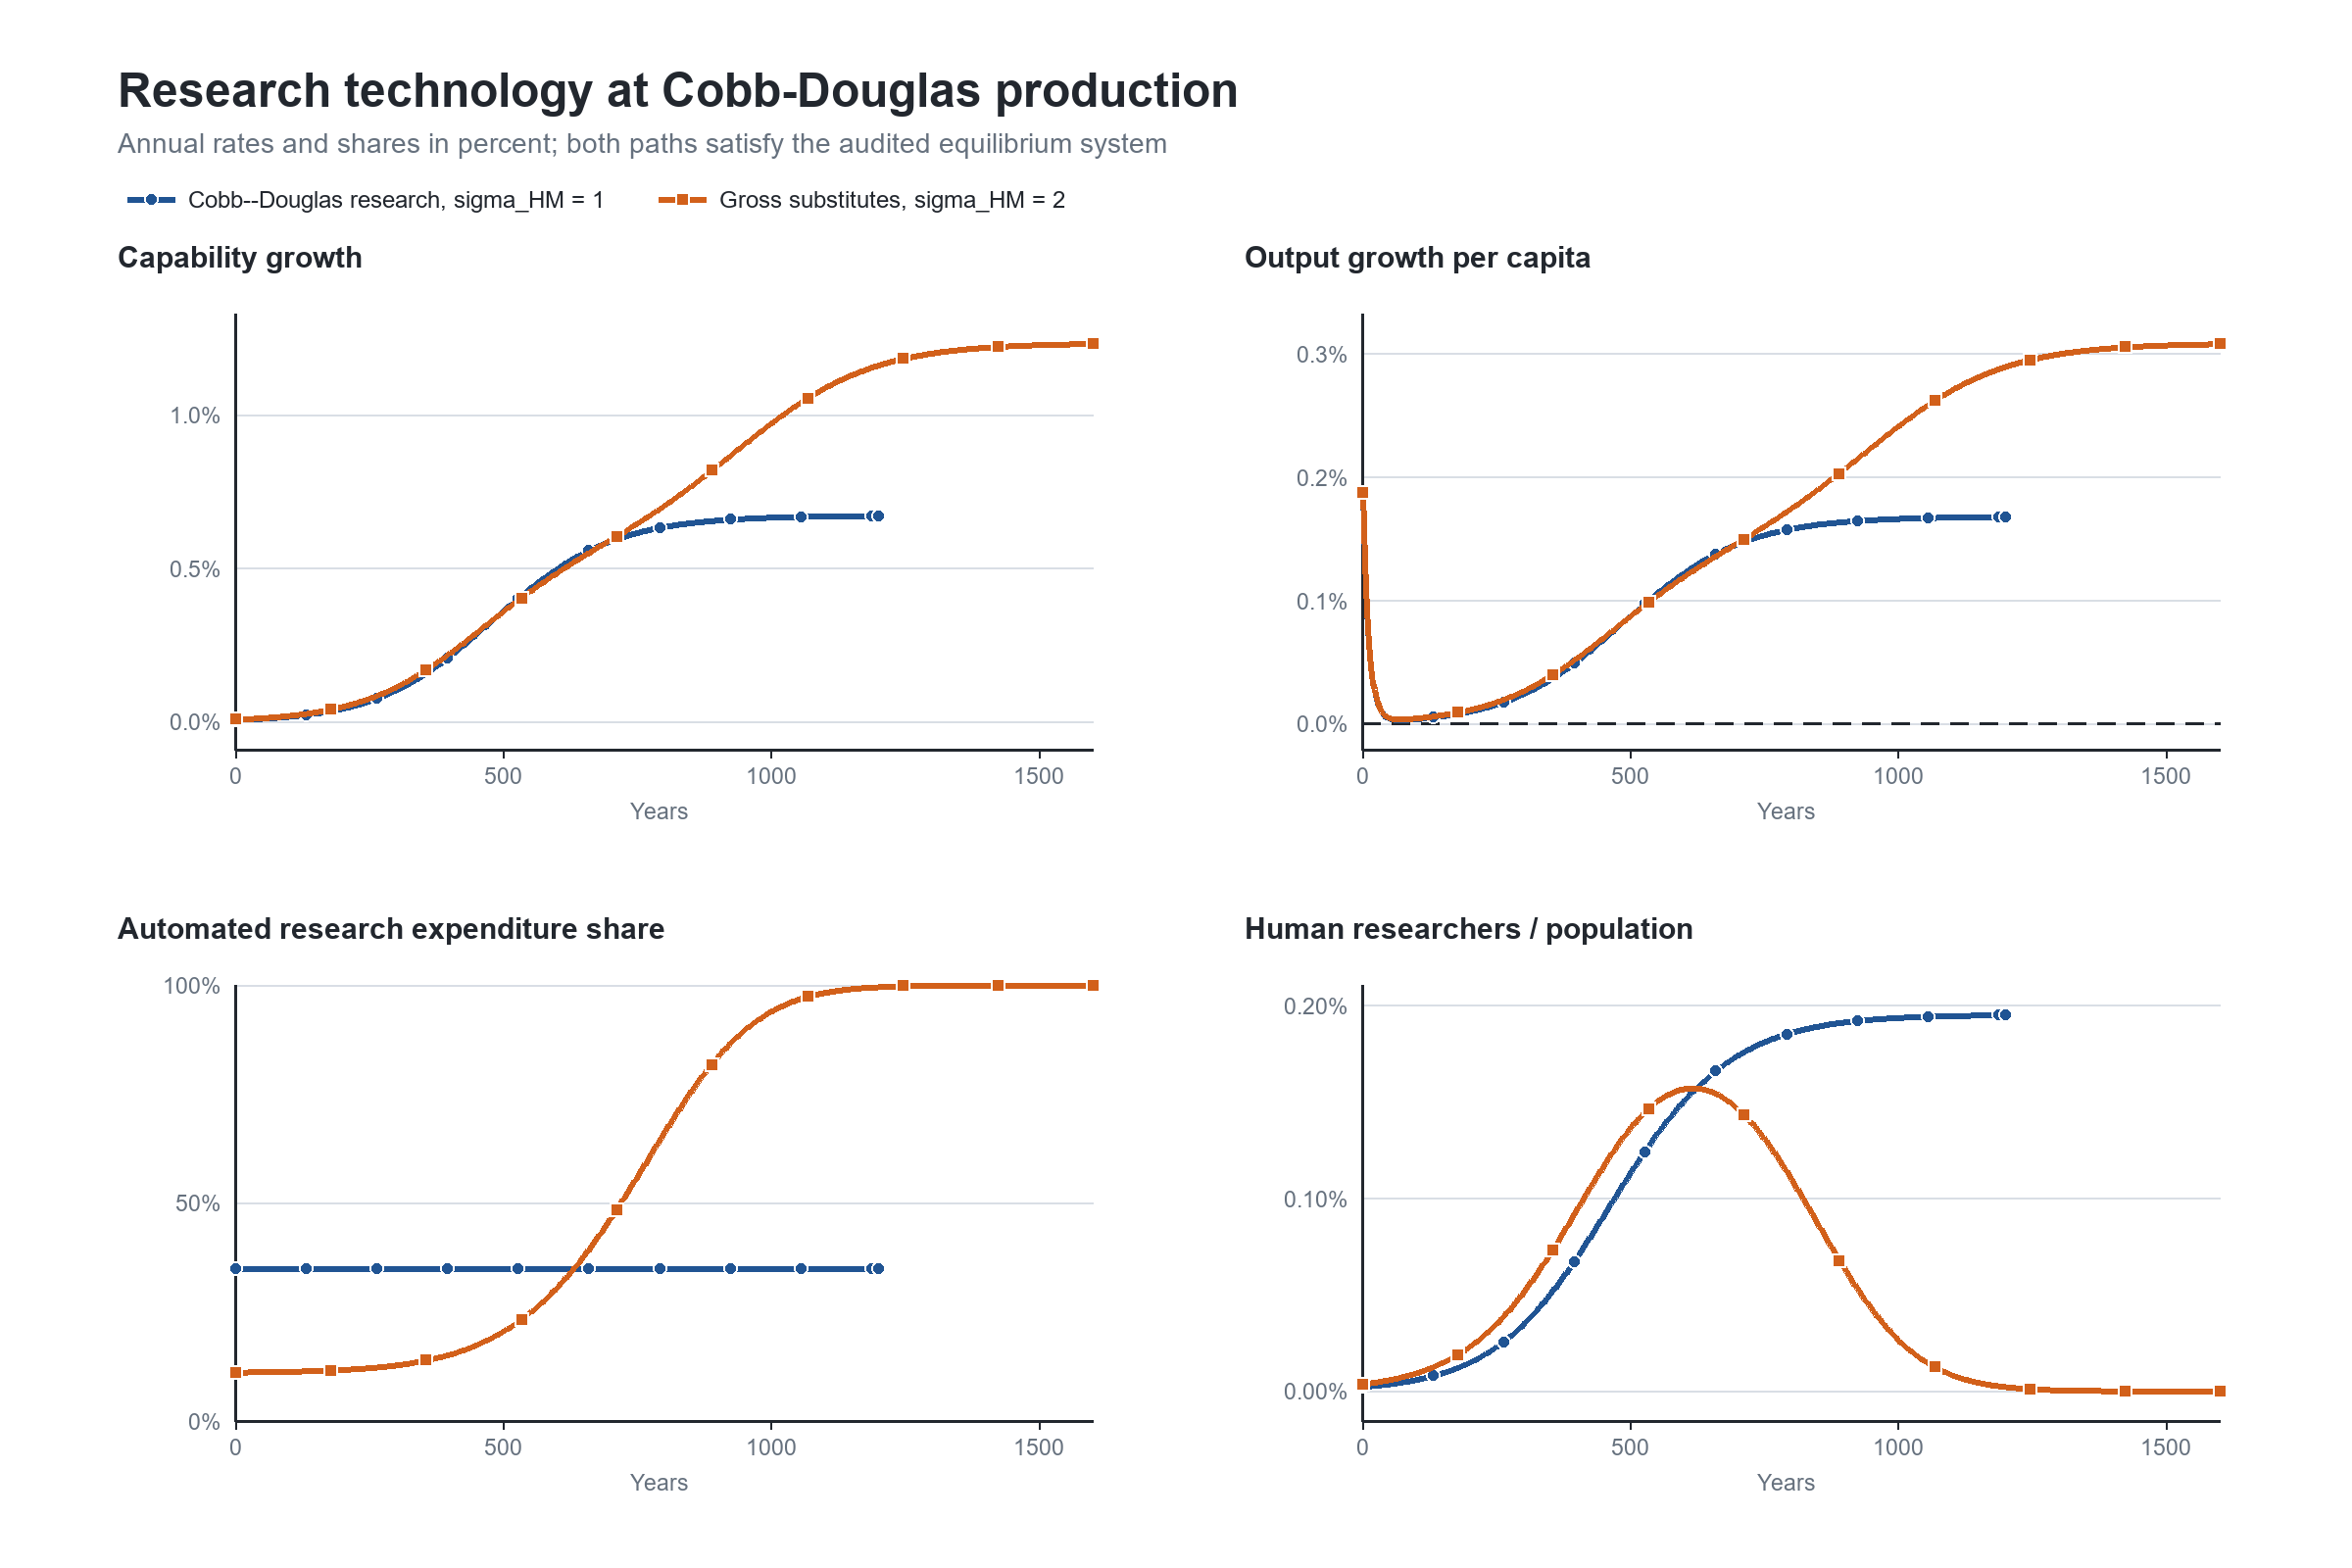
\includegraphics[width=\textwidth]{figures_axm/axm_research_technology_comparison.png}
\caption{Research substitution and the unit-elasticity balanced-growth limit.
Both lines are perfect-foresight equilibrium paths.}
\label{fig:axm-research-comparison}
\end{figure}

The human-research transition contains a result that is hidden by the limiting
research share. With \(\sigma_{HM}=2\), the fraction of the population working in
AI research first rises and later falls toward zero. AI research can therefore
employ more people during the transition even while it becomes progressively more
automated. Under Cobb--Douglas research, the human-research population share
instead converges to a positive constant.

Figure \ref{fig:axm-wages} shows that the distinction between factor prices and
factor shares already matters on these balanced-growth transitions. The real wage
eventually grows at the same rate as output per person, as Proposition
\ref{prop:axm-cd-bgp} requires. The production labor share is fixed by the
Cobb--Douglas final-production technology, while total labor income also includes
human researchers and therefore moves during the research-automation transition.

\begin{figure}[H]
\centering
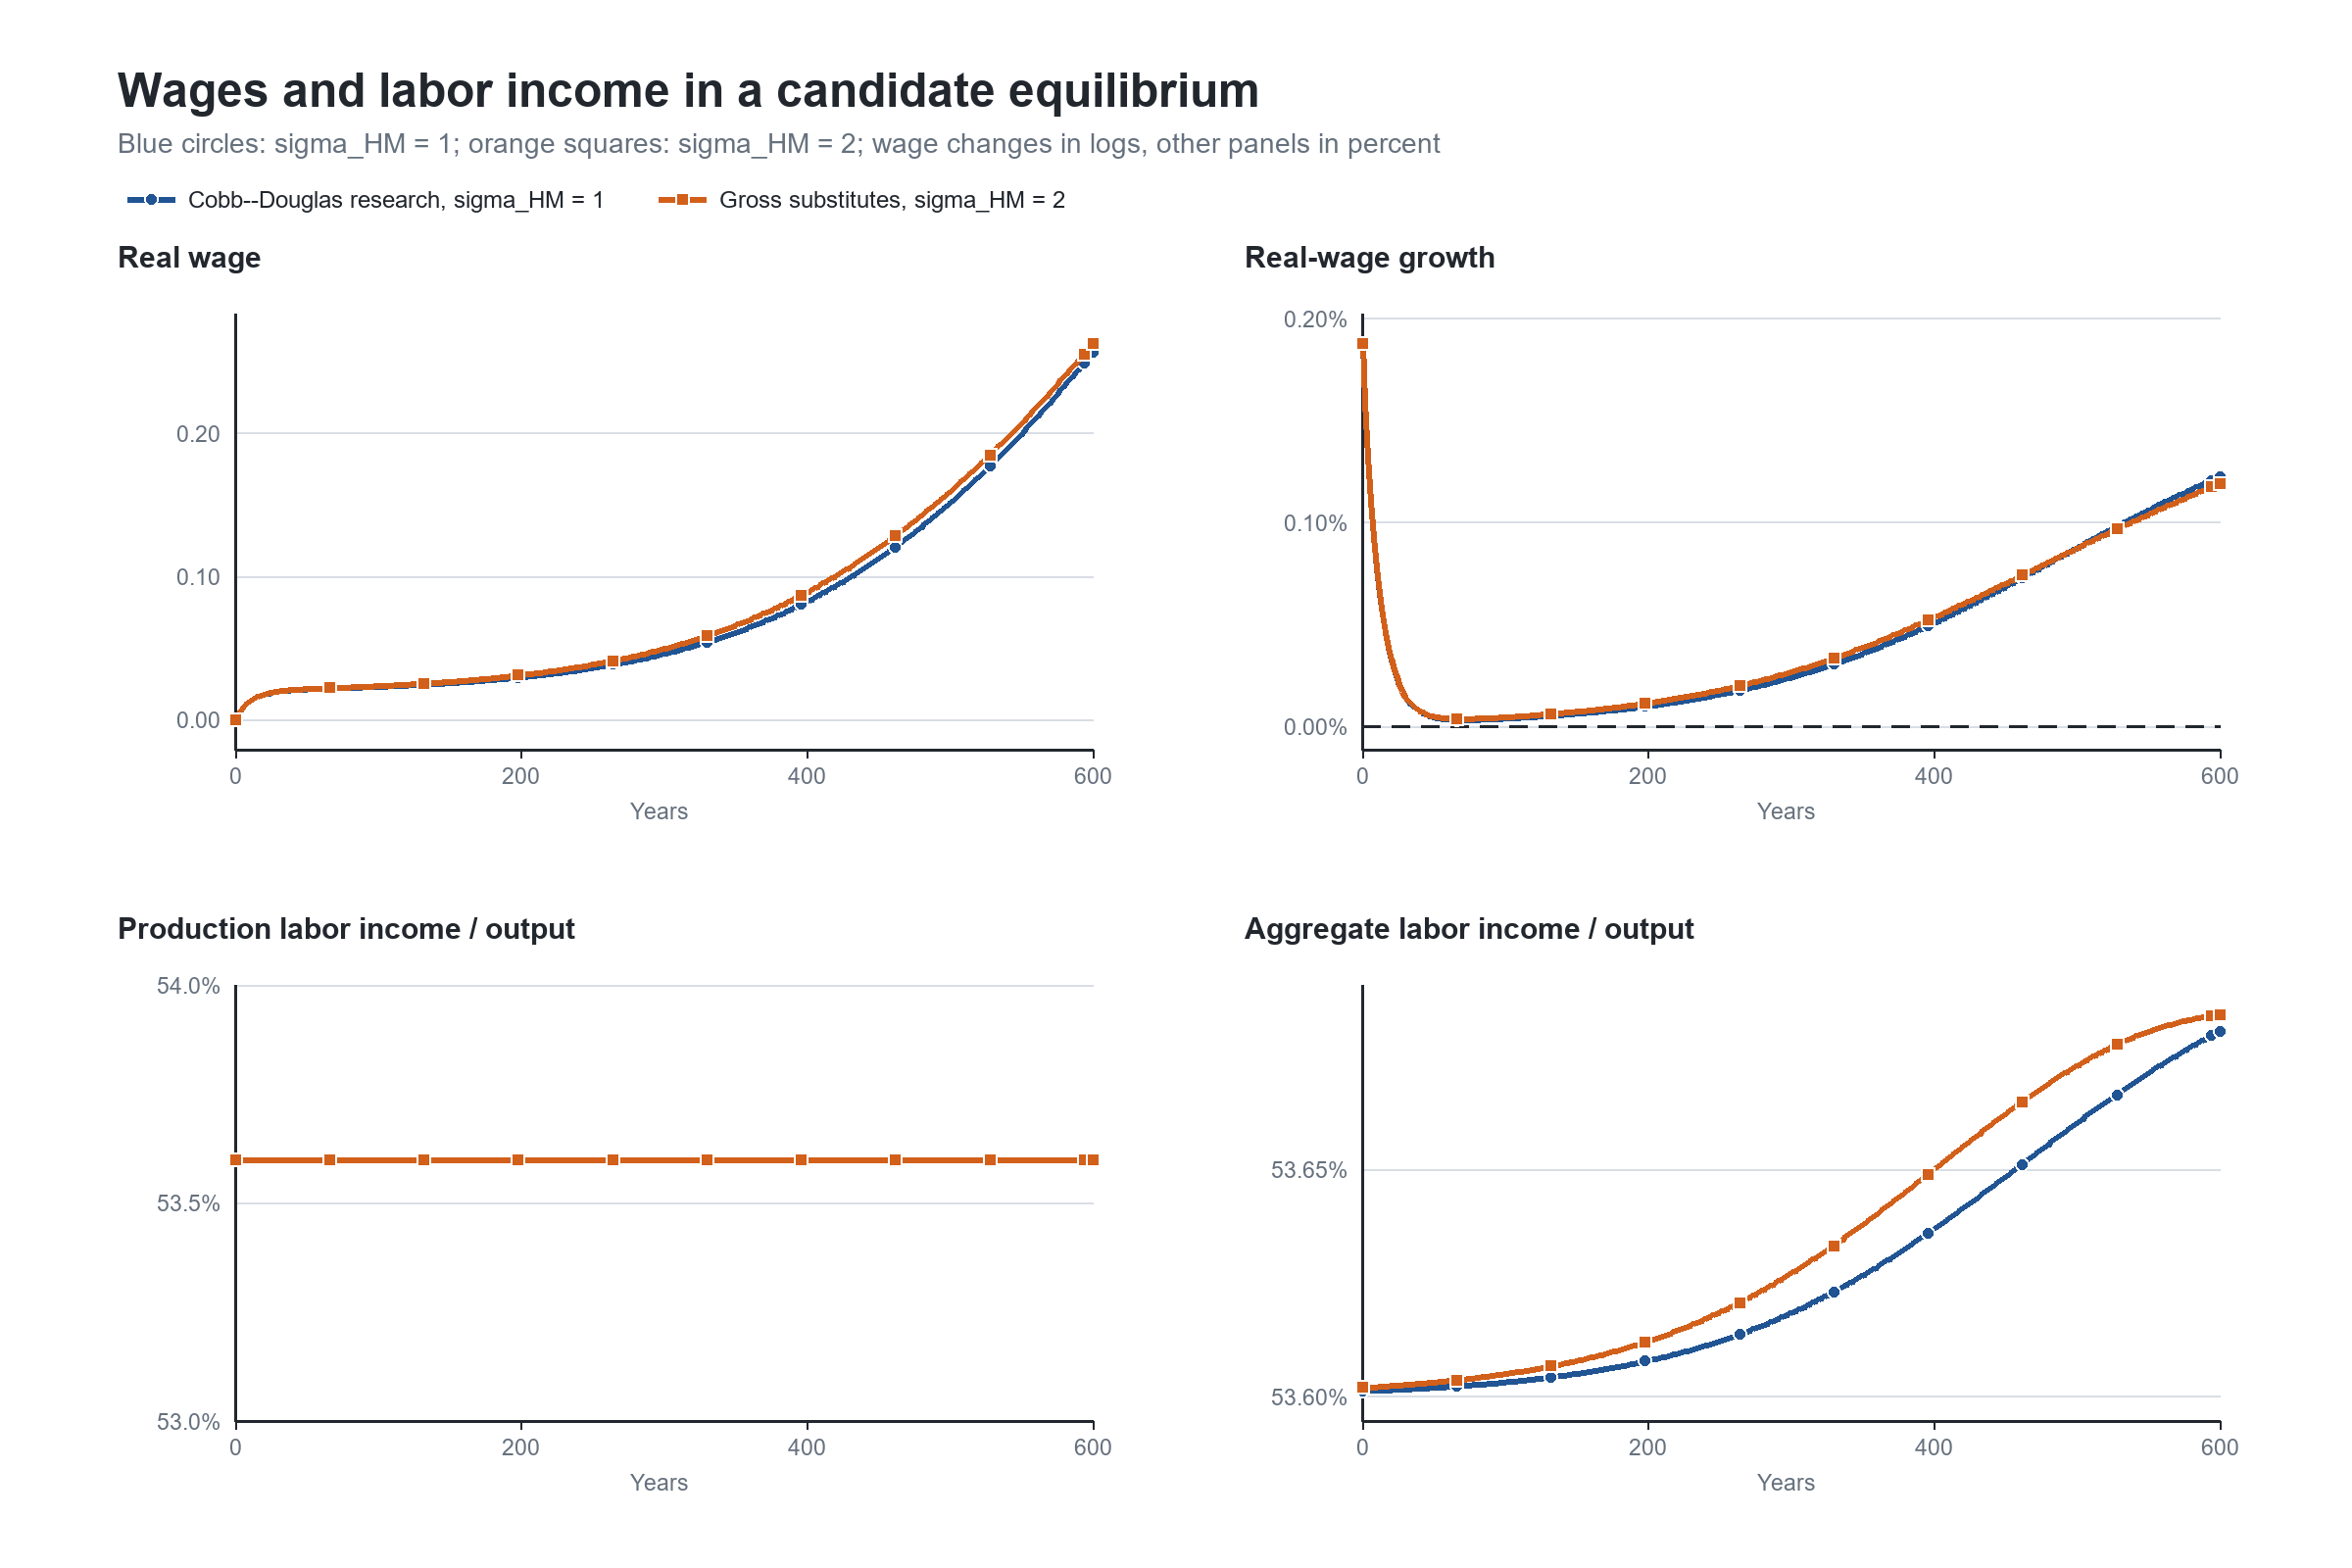
\includegraphics[width=\textwidth]{figures_axm/axm_wages_and_factor_shares.png}
\caption{Real wages and labor income. Both paths satisfy the canonical
equilibrium system.}
\label{fig:axm-wages}
\end{figure}

Figure \ref{fig:axm-research-chain} separates raw research compute \(M\), the
automated services \(AM\), human research \(H\), and effective research \(E\).
This decomposition is essential for interpreting the new specification. Research
compute can grow at one rate while the services produced by that compute grow
faster because capability is improving.

\begin{figure}[H]
\centering
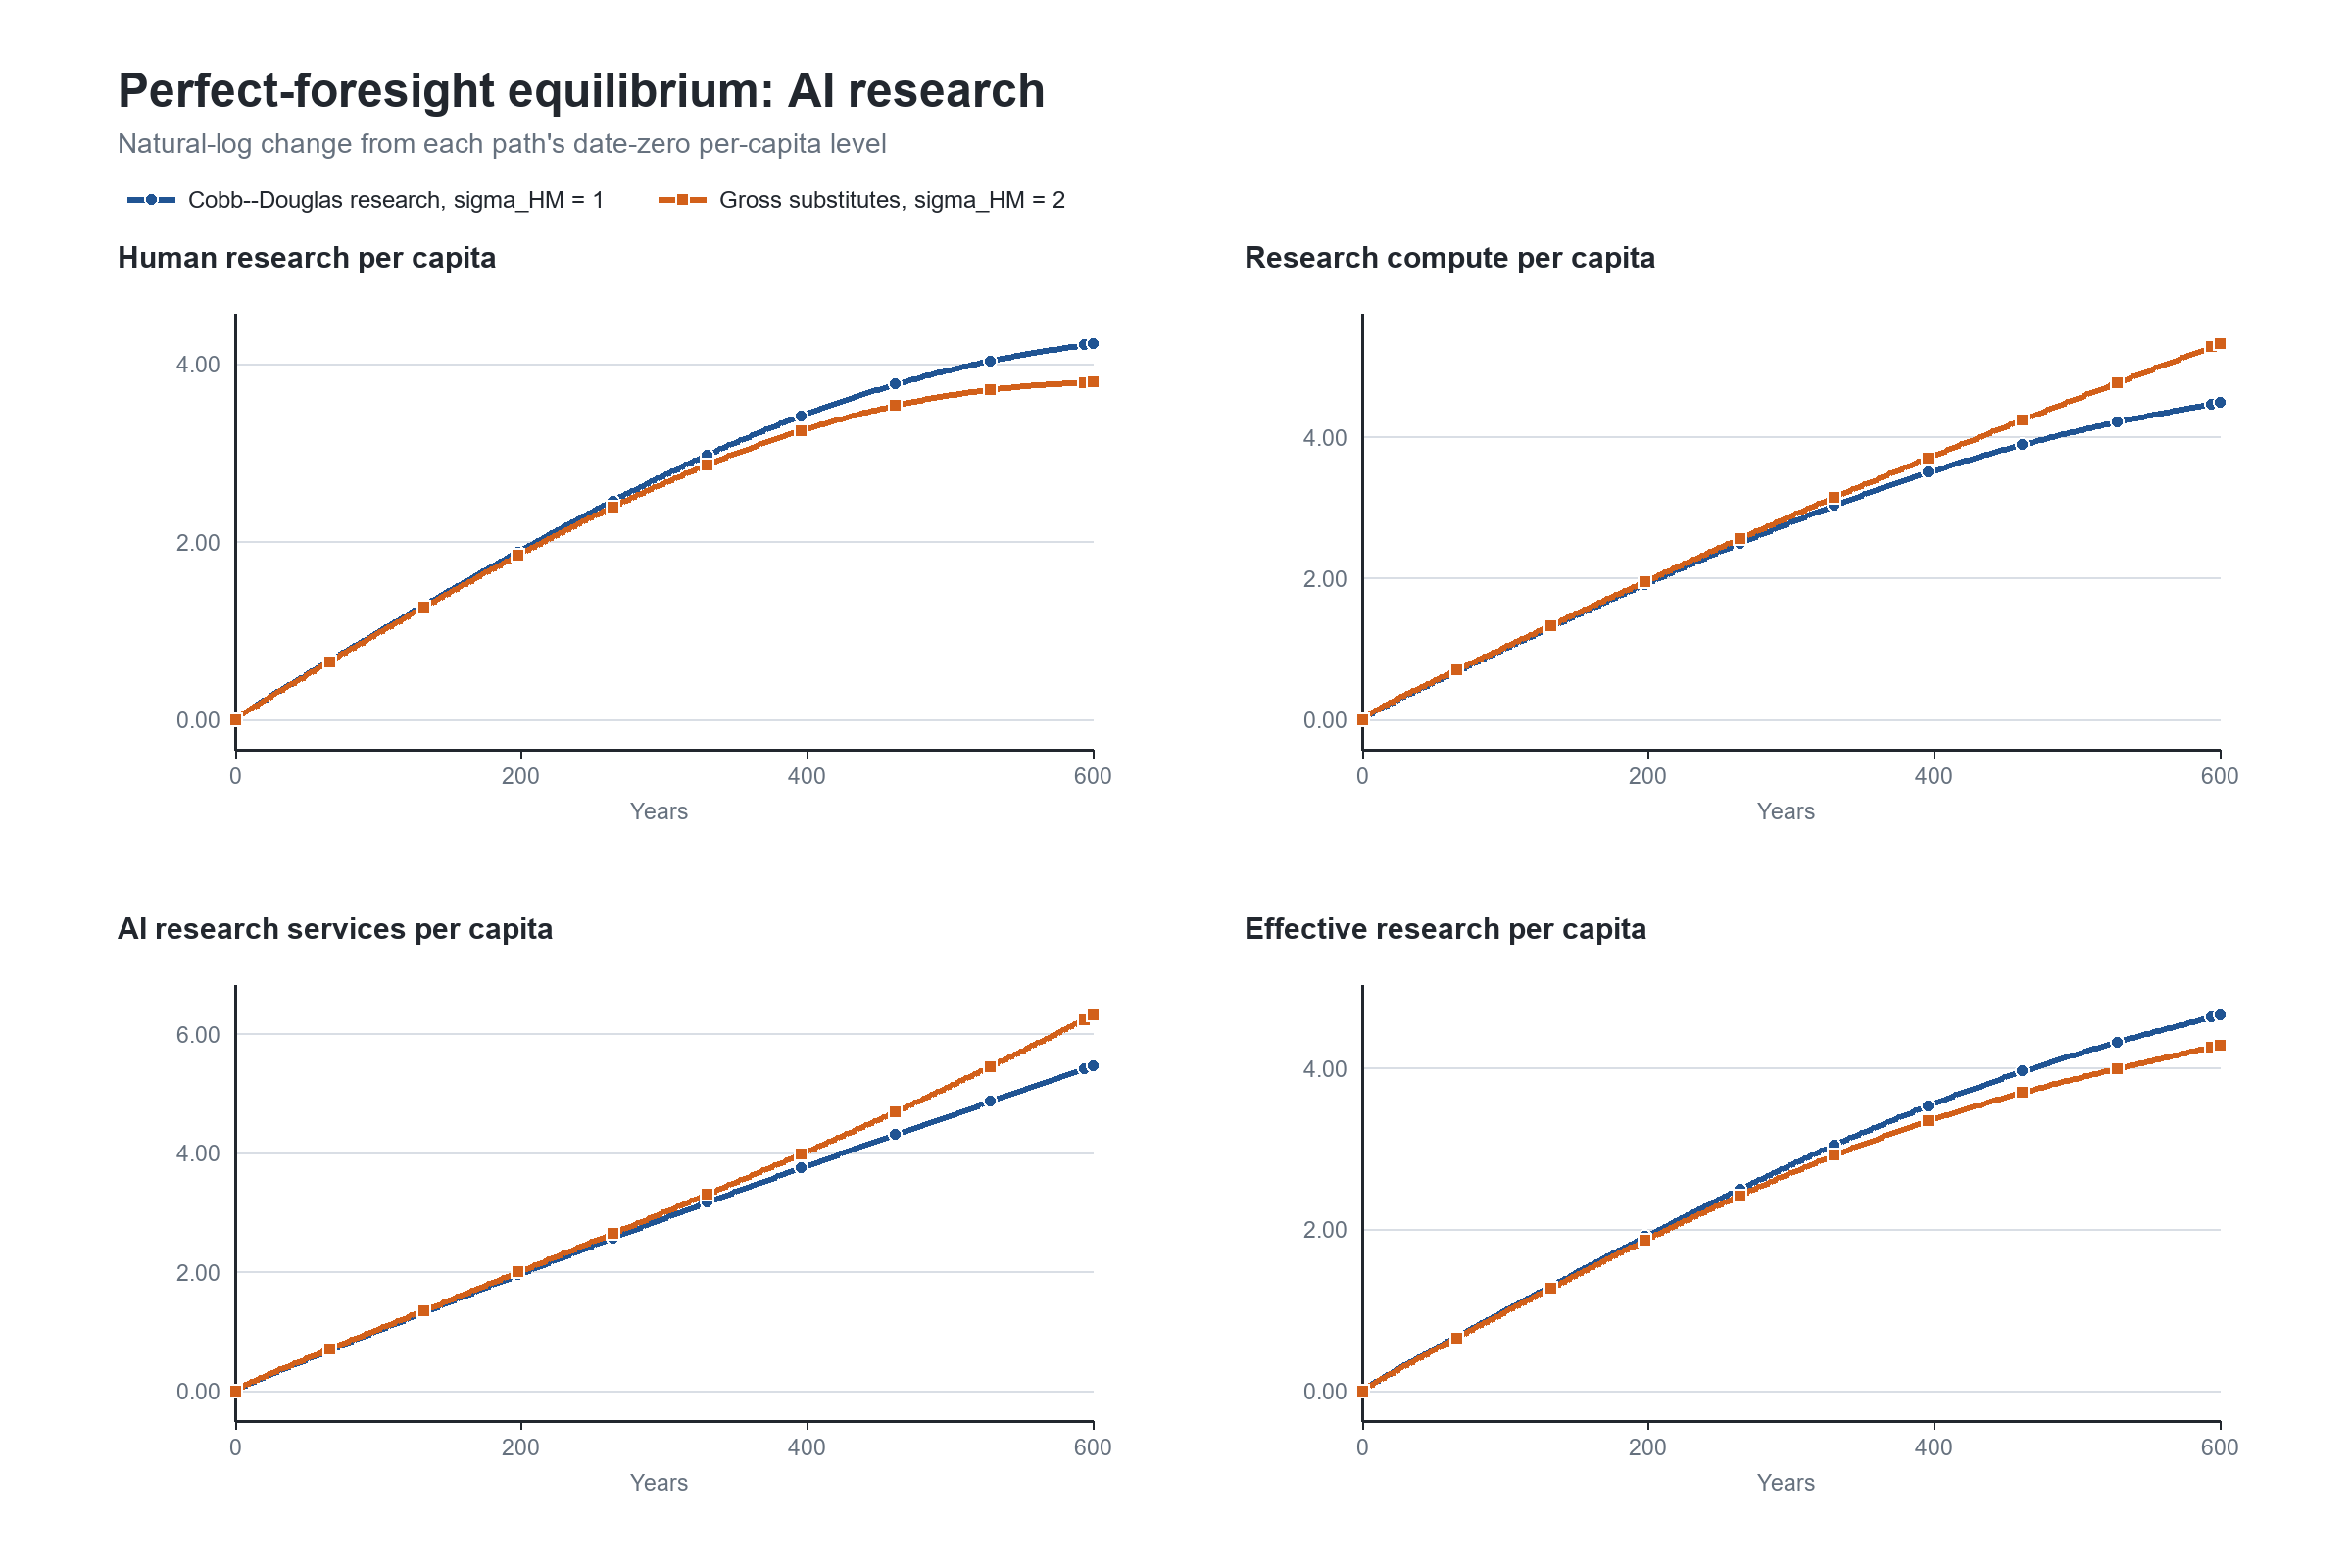
\includegraphics[width=\textwidth]{figures_axm/axm_equilibrium_research_chain.png}
\caption{The AI-research chain. The vertical axes report natural-log changes from
each path's date-zero per-capita level.}
\label{fig:axm-research-chain}
\end{figure}

\subsection{Equilibrium audit}

Table \ref{tab:axm-residuals} reports the numerical audit. The static identities
and first-order conditions are satisfied to approximately machine precision.
The larger numbers are collocation errors in the differential equations and
remain close to \(10^{-5}\). The terminal rates are also close to the analytical
targets despite solving the transition rather than imposing the entire
balanced-growth path.

\begin{table}[H]
\centering
\caption{Equilibrium-path diagnostics}
\label{tab:axm-residuals}
\begin{tabular}{lcc}
\toprule
Diagnostic & \(\sigma_{HM}=1\) & \(\sigma_{HM}=2\)\\
\midrule
Maximum goods-market residual & \(2.2\times10^{-16}\) & \(2.2\times10^{-16}\)\\
Maximum labor-market residual & \(8.9\times10^{-16}\) & \(1.8\times10^{-15}\)\\
Maximum research-FOC log error & \(3.6\times10^{-13}\) & \(1.3\times10^{-11}\)\\
Maximum dynamic path residual & \(4.4\times10^{-6}\) & \(1.2\times10^{-5}\)\\
Terminal automated research share & 0.3500 & 0.99999\\
\bottomrule
\end{tabular}
\end{table}

\subsection{Gross substitution in final production}

For \(\sigma_{XL}>1\), a conventional terminal balanced-growth condition would
contradict Proposition \ref{prop:axm-no-bgp}. We therefore use a separate
free-boundary algorithm that terminates at a large value of \(Y/K\) and imposes
the limiting ratios in Conditional Result \ref{prop:axm-singular-limit}. A path is
reported only after convergence across progressively larger terminal boundaries
and after the same equilibrium-residual audit used above. This prevents a
finite-horizon initial-value path from being mislabeled as an infinite-horizon
equilibrium.

The robust qualitative prediction is analytical: the economy can remain close to
ordinary growth while \(Y/K\) is moderate, but growth and the return to capital
rise together once the AI-dominated scaling becomes quantitatively important. We
do not report a high-substitution curve in the present numerical set. Fixed-horizon
solutions satisfy the local equilibrium equations, but the free-boundary
continuation has not yet passed the convergence test across increasingly distant
terminal boundaries. Presenting such a curve as an equilibrium transition would
therefore overstate what has been verified. The analytical nonexistence and
limiting-ratio results do not depend on that unfinished numerical exercise.
